%%%%%%%%%%%%  Generated using docx2latex.com  %%%%%%%%%%%%%%

%%%%%%%%%%%%  v2.0.0-beta  %%%%%%%%%%%%%%

% This template is made using Docx2Latex add-on for Google
% Docs, Refer following videos 
% Getting started : 
% 
% How to use add on :
% 
\documentclass[12pt]{article}

 %%%%%%%%%%%%  Include Packages  %%%%%%%%%%%%%%


\usepackage{txfonts}
\usepackage{setspace}
\usepackage[a4paper,left=1.0in,right=1.0in,top=1.0in,bottom=1.0in,headheight=1in]{geometry}
\usepackage{fancyhdr}
\fancypagestyle{plain}{%
 \fancyhf{}
 \fancyfoot[CE]{Pune Institute of Computer Technology, Department of Computer Engineering 2017-18}
 \fancyfoot[RE]{\thepage}
}
\pagestyle{fancy}
\fancyhead{}
\renewcommand{\headrulewidth}{0pt}
\footskip = 0.625in
\cfoot{}
\rfoot{}
% removes the horizontal line in certificate
\setlength\arrayrulewidth{0pt}
% Blank space below is for aesthetics purpose only
\usepackage{amsmath}
\usepackage{latexsym}
\usepackage{amsfonts}
\usepackage[normalem]{ulem}
\usepackage{soul}
\usepackage{array}
\usepackage{amssymb}
\usepackage{extarrows}
\usepackage{graphicx}
\usepackage[backend=biber,
style=numeric,
sorting=none,
isbn=false,
doi=false,
url=false,
]{biblatex}\addbibresource{bibliography.bib}

\usepackage{subfig}
\usepackage{wrapfig}
\usepackage{wasysym}
\usepackage{enumitem}
\usepackage{adjustbox}
\usepackage{ragged2e}
\usepackage[svgnames,table]{xcolor}
\usepackage{tikz}
\usepackage{longtable}
\usepackage{changepage}
\usepackage{hhline}
\usepackage{multicol}
\usepackage{tabto}
\usepackage{float}
\usepackage{multirow}
\usepackage{makecell}
\usepackage[toc,page]{appendix}
\usepackage[hidelinks]{hyperref}
\usetikzlibrary{shapes.symbols,shapes.geometric,shadows,arrows.meta}
\tikzset{>={Latex[width=1.5mm,length=2mm]}}
\usepackage{flowchart}\usepackage[utf8]{inputenc}
\usepackage[T1]{fontenc}
\TabPositions{0.5in,1.0in,1.5in,2.0in,2.5in,3.0in,3.5in,4.0in,4.5in,5.0in,5.5in,6.0in,}
\usepackage{biblatex}
\addbibresource{bibliography.bib}


\urlstyle{same}

\renewcommand{\_}{\kern-1.5pt\textunderscore\kern-1.5pt}

 %%%%%%%%%%%%  Set Depths for Sections  %%%%%%%%%%%%%%

% 1) Section
% 1.1) SubSection
% 1.1.1) SubSubSection
% 1.1.1.1) Paragraph
% 1.1.1.1.1) Subparagraph


\setcounter{tocdepth}{5}
\setcounter{secnumdepth}{5}


 %%%%%%%%%%%%  Set Depths for Nested Lists created by \begin{enumerate}  %%%%%%%%%%%%%%


\setlistdepth{9}
\renewlist{enumerate}{enumerate}{9}
		\setlist[enumerate,1]{label=\arabic*)}
		\setlist[enumerate,2]{label=\alph*)}
		\setlist[enumerate,3]{label=(\roman*)}
		\setlist[enumerate,4]{label=(\arabic*)}
		\setlist[enumerate,5]{label=(\Alph*)}
		\setlist[enumerate,6]{label=(\Roman*)}
		\setlist[enumerate,7]{label=\arabic*}
		\setlist[enumerate,8]{label=\alph*}
		\setlist[enumerate,9]{label=\roman*}

\renewlist{itemize}{itemize}{9}
		\setlist[itemize]{label=$\cdot$}
		\setlist[itemize,1]{label=\textbullet}
		\setlist[itemize,2]{label=$\circ$}
		\setlist[itemize,3]{label=$\ast$}
		\setlist[itemize,4]{label=$\dagger$}
		\setlist[itemize,5]{label=$\triangleright$}
		\setlist[itemize,6]{label=$\bigstar$}
		\setlist[itemize,7]{label=$\blacklozenge$}
		\setlist[itemize,8]{label=$\prime$}

\setlength{\topsep}{0pt}\setlength{\parindent}{0pt}

 %%%%%%%%%%%%  This sets linespacing (verticle gap between Lines) Default=1 %%%%%%%%%%%%%%


\renewcommand{\arraystretch}{1.3}


%%%%%%%%%%%%%%%%%%%% Document code starts here %%%%%%%%%%%%%%%%%%%%



\begin{document}

\vspace{\baselineskip}
\begin{Center}
{\fontsize{14pt}{16.8pt}\selectfont \textbf{PUNE INSTITUTE OF COMPUTER TECHNOLOGY,}\par}
\end{Center}\par

\begin{Center}
{\fontsize{14pt}{16.8pt}\selectfont \textbf{DHANKAWADI PUNE-43.}\par}
\end{Center}\par

\begin{Center}
{\fontsize{26pt}{31.2pt}\selectfont \textbf{\textit{A Seminar Report}}\par}
\end{Center}\par

\begin{Center}
\textbf{\textit{ }\ \ \ \  }{\fontsize{24pt}{28.8pt}\selectfont \textbf{\textit{\ On  }\  }\par}
\end{Center}\par

\begin{Center}
{\fontsize{16pt}{19.2pt}\selectfont \textbf{ Similarity Search Algorithms on Embeddings }\par}
\end{Center}\par

\begin{Center}
{\fontsize{16pt}{19.2pt}\selectfont \textbf{in Face Recognition}\par}
\end{Center}\par

\begin{Center}
{\fontsize{14pt}{16.8pt}\selectfont  \par}
\end{Center}\par

\begin{Center}
{\fontsize{14pt}{16.8pt}\selectfont SUBMITTED BY\par}
\end{Center}\par

\begin{Center}
{\fontsize{14pt}{16.8pt}\selectfont  \par}
\end{Center}\par

\begin{Center}
{\fontsize{16pt}{19.2pt}\selectfont \textbf{NAME: Apoorv Dixit}\par}
\end{Center}\par

\begin{Center}
{\fontsize{16pt}{19.2pt}\selectfont \textbf{ROLL NO: 31106}\par}
\end{Center}\par

\begin{Center}
{\fontsize{16pt}{19.2pt}\selectfont \textbf{CLASS: TE-1}\par}
\end{Center}\par

\begin{Center}
{\fontsize{7pt}{8.4pt}\selectfont \textbf{ }\par}
\end{Center}\par

\begin{Center}
{\fontsize{14pt}{16.8pt}\selectfont GUIDED BY\par}
\end{Center}\par

\begin{Center}
{\fontsize{16pt}{19.2pt}\selectfont \textbf{PROF. P. S. Vidap}\par}
\end{Center}\par



%%%%%%%%%%%%%%%%%%%% Figure/Image No: 1 starts here %%%%%%%%%%%%%%%%%%%%

\begin{figure}[H]
	\begin{Center}
		
\includegraphics[width=1.57in,height=1.57in]{./media/image2.jpg}
	\end{Center}
\end{figure}


%%%%%%%%%%%%%%%%%%%% Figure/Image No: 1 Ends here %%%%%%%%%%%%%%%%%%%%

\tab \par

 \par

 \par

 \par

\begin{Center}
{\fontsize{20pt}{24.0pt}\selectfont \textbf{COMPUTER ENGINEERING DEPARTMENT}\par}
\end{Center}\par

\begin{Center}
{\fontsize{20pt}{24.0pt}\selectfont \textbf{Academic Year: 2019-20}\par}

 %%%%%%%%%%%%  Starting New Page here %%%%%%%%%%%%%%

\newpage

\end{Center}\par


\vspace{\baselineskip}
\begin{Center}
{\fontsize{20pt}{24.0pt}\selectfont \textbf{ }\par}
\end{Center}\par

\begin{Center}
{\fontsize{14pt}{16.8pt}\selectfont \textbf{PUNE INSTITUTE OF COMPUTER TECHNOLOGY,}\par}
\end{Center}\par

\begin{Center}
{\fontsize{14pt}{16.8pt}\selectfont \textbf{DHANKAWADI PUNE-43.}\par}
\end{Center}\par


\vspace{\baselineskip}
\begin{Center}
{\fontsize{26pt}{31.2pt}\selectfont \textbf{\textit{CERTIFICATE}}{\fontsize{14pt}{16.8pt}\selectfont  \par}\par}
\end{Center}\par



%%%%%%%%%%%%%%%%%%%% Figure/Image No: 2 starts here %%%%%%%%%%%%%%%%%%%%

\begin{figure}[H]
	\begin{Center}
		
\includegraphics[width=1.57in,height=1.57in]{./media/image2.jpg}
	\end{Center}
\end{figure}


%%%%%%%%%%%%%%%%%%%% Figure/Image No: 2 Ends here %%%%%%%%%%%%%%%%%%%%

\begin{Center}
{\fontsize{14pt}{16.8pt}\selectfont  \par}
\end{Center}\par

\begin{justify}
{\fontsize{18pt}{21.6pt}\selectfont This is to certify that {\fontsize{20pt}{24.0pt}\selectfont Mr.\textit{ \textbf{\uline{Apoorv Dixit}} }{\fontsize{18pt}{21.6pt}\selectfont \textit{, R}oll No\textbf{. }{\fontsize{20pt}{24.0pt}\selectfont \textbf{\uline{31106}}{\fontsize{18pt}{21.6pt}\selectfont \  a student of T.E. (Computer Engineering Department) Batch 2019-2020, has satisfactorily completed a seminar report on $``${\fontsize{16pt}{19.2pt}\selectfont \textbf{Similarity Search Algorithms on Embeddings in Face Recognition$"$ }{\fontsize{18pt}{21.6pt}\selectfont  \tab under the guidance of \uline{Prof. P. S.Vidap} towards the partial fulfillment of the third year Computer Engineering Semester II of Pune University.\par}\par}\par}\par}\par}\par}\par}
\end{justify}\par

\begin{justify}
{\fontsize{18pt}{21.6pt}\selectfont  \par}
\end{justify}\par


\vspace{\baselineskip}

\vspace{\baselineskip}

\vspace{\baselineskip}


%%%%%%%%%%%%%%%%%%%% Table No: 1 starts here %%%%%%%%%%%%%%%%%%%%


\begin{table}[H]
 			\centering
\begin{tabular}{p{2.94in}p{2.94in}}
\hline
%row no:1
\multicolumn{1}{p{2.94in}}{Prof. P. S. Vidap } & 
\multicolumn{1}{p{2.94in}}{\Centering Prof.\ M.S.Takalikar  } \\
\hhline{~~}
%row no:2
\multicolumn{1}{p{2.94in}}{\textbf{Internal Guide}\textit{\  }} & 
\multicolumn{1}{p{2.94in}}{\Centering \textbf{Head of Department\textit{,}}} \\
\hhline{~~}
%row no:3
\multicolumn{1}{p{2.94in}}{} & 
\multicolumn{1}{p{2.94in}}{\Centering \textbf{Computer Engineering} } \\
\hhline{~~}

\end{tabular}
 \end{table}


%%%%%%%%%%%%%%%%%%%% Table No: 1 ends here %%%%%%%%%%%%%%%%%%%%


\vspace{\baselineskip}
\setlength{\parskip}{6.0pt}
{\fontsize{14pt}{16.8pt}\selectfont \textbf{Date:}\par}\par

{\fontsize{14pt}{16.8pt}\selectfont \textbf{Place:}\par}

 %%%%%%%%%%%%  Starting New Page here %%%%%%%%%%%%%%
 
\newpage

\pagenumbering{Roman}
\section*{ACKNOWLEDGEMENT}


\vspace{0.25cm}
\par 
 \hspace{1cm}
I would like to extend my sincerest gratitude to my guide Prof. P.S. Vidap for providing me with the necessary resources as well as her invaluable insights. This seminar would not have been possible without her constant support. She has been instrumental in making this seminar a grand success.

\newpage
\begin{center}
\section*{SIMILARITY SEARCH ALGORITHMS ON \\EMBEDDINGS IN FACE RECOGNITION}
\end{center}
\par

 \par


\vspace{\baselineskip}
{\fontsize{14pt}{16.8pt}\selectfont \textbf{\textit{Abstract:}}\par}\par

\setlength{\parskip}{12.0pt}
\begin{justify}
\textit{Face Recognition is a challenging task in computer vision in which researchers from all over the world have made great strides owing to the development of more robust and accurate deep learning models. These frameworks have come a long way from hand engineered systems to the end-to-end mapped models that are state of the art today. However, implementing faster similarity search of face features is an increasingly important problem. There is a dire need to address this issue in order to make the face recognition pipelines scalable and more suited for real time applications. This seminar aims to benchmark different similarity search algorithms on face embeddings generated from a standard face dataset. The benchmarking will help other users choose a nearest neighbour search method for their face recognition models.}
\end{justify}\par

\begin{justify}
{\fontsize{14pt}{16.8pt}\selectfont \textbf{\textit{ }}\par}
\end{justify}\par

\begin{justify}
{\fontsize{14pt}{16.8pt}\selectfont \textbf{\textit{Keywords}}\textit{:} \textit{Face recognition, computer vision, deep learning model, nearest neighbor search, embeddings, similarity search, benchmark.}\par}
\end{justify}\par
\newpage

\setlength{\parskip}{6.0pt}

 \par


% Following code generates Table Of Contents
% List Of Figures
% and Table Of Tables
\tableofcontents
\newpage
\listoffigures
\listoftables
\newpage
\setlength\arrayrulewidth{0.4pt}
\renewcommand{\headrulewidth}{0.4pt}
\pagenumbering{arabic}
\vspace{\baselineskip}

\vspace{\baselineskip}

\frontmatter
\chead{Similarity Search Algorithms on Embedding in Face Recognition}
\rhead{\thepage}
\rfoot{``Department of Computer Engineering, PICT Pune” \ \ \ \ \ P:F/SMR-UG/08/R0}
\linespread{1.25}

\section*{1\hspace*{10pt}INTRODUCTION}
\addcontentsline{toc}{section}{1\hspace*{10pt}INTRODUCTION}
\begin{justify}
Face Recognition is the task of identifying a person from either a digital image or a frame from a video. This task is typically accomplished by obtaining facial features of a face from a given image and subsequently comparing it with other faces stored in a database. It finds its application in a wide variety of fields like robotics, access controls in security systems, commercial identification, marketing tool, human computer interaction, video surveillance, biometrics and many more. Face Recognition’s contactless and non-invasive process is what sets it apart from other biometric technologies like iris recognition and fingerprint recognition.
\end{justify}\par

\begin{justify}
Face Recognition is a task that can be performed trivially by humans, but can prove to be a daunting challenge for machines. It has remained so for computer vision problems until recently. There have been major strides in the development of more accurate and robust systems in face recognition owing to the advent of artificial intelligence in the past two decades. We have come a long way from the hand engineered models used in the beginning of the 21\textsuperscript{st}\ century to the deep learning pipelines that are pretty much the state of the art today. It is only in recent times that these state of the art models have matched, if not surpassed, the human accuracy. The deep learning systems employed take into consideration various variable conditions like light textures, pose and orientation of  the person’s face, age of the person, the varying facial hair and much more.
\end{justify}\par

\setlength{\parskip}{12.0pt}
\begin{justify}
Face Recognition Pipelines are primarily broken down into the following major subtasks – Face Detection, Face Alignment, Feature Extraction and finally, the recognition task. The Modern deep learning pipelines for facial recognition systems deploy deep learning models for the first three subtasks, and use an Approximate Nearest Neighbour Search Algorithm (ANN) for the recognition. This report will be focusing on face embeddings and various ANN, which will cater to Feature Extraction and Recognition respectively.
\end{justify}\par

\begin{justify}


%%%%%%%%%%%%%%%%%%%% Figure/Image No: 3 starts here %%%%%%%%%%%%%%%%%%%%

\begin{figure}[H]
	\begin{FlushLeft}		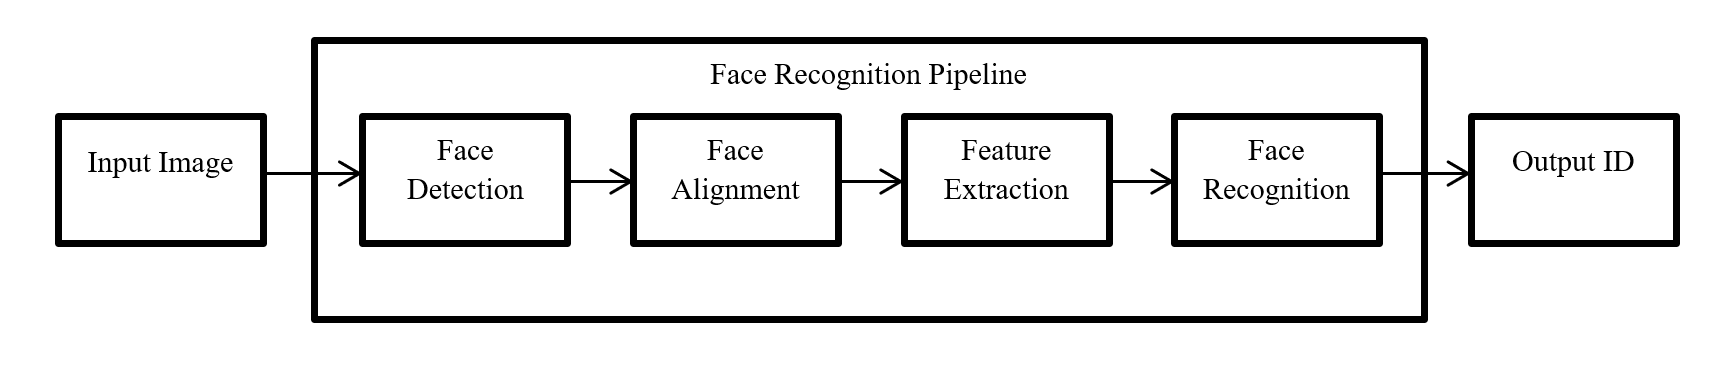
\includegraphics[width=6.27in,height=1.36in]{./media/image6.png}
		\caption{Face Recognition Pipeline Architecture}
		\label{fig:Face_Recognition_Pipeline_Architecture}
	\end{FlushLeft}\end{figure}


%%%%%%%%%%%%%%%%%%%% Figure/Image No: 3 Ends here %%%%%%%%%%%%%%%%%%%%

\\

\end{justify}\par

\setlength{\parskip}{6.0pt}
\subsection*{1.1\hspace*{10pt}Motivation}
\addcontentsline{toc}{subsection}{1.1\hspace*{10pt}Motivation}
\begin{justify}
While accuracy is not that big of a problem in Face Recognition Systems anymore, making them more suited for real time tasks is. The deep learning models that we see today have been trained on millions of faces. The memory footprint of these models is way too heavy to be used for real time systems. Moreover deep learning pipelines are composed of more than one deep learning model, to perform the different subtasks like Face Detection, Face Alignment and Feature Extraction. This makes them too slow for achieving the overall objective. 
\end{justify}\par

\begin{justify}
This issue can be tackled in two ways. The first way is to design a more light weight deep learning model for feature extraction. The second way is to select a fast ANN for the final recognition subtask. This final subtask involves comparing the extracted features of the face obtained with that of faces stored in a database. This subtask returns the ID of the person the face resembles the closest to, thereby recognizing the person. The database typically stores the extracted features of faces rather than the images of the faces themselves. The comparison is done by an ANN.
\end{justify}\par

\subsection*{1.2\hspace*{10pt}Literature Survey}
\addcontentsline{toc}{subsection}{1.2\hspace*{10pt}Literature Survey}
1.2.1\tab \textbf{ANN-Benchmarks: A Benchmarking Tool for Approximate Nearest Neighbor Algorithms }\par
This paper talks about ANN-Benchmarks \cite{aumuller2017ann} , a tool for evaluating the performance of in-memory approximate nearest neighbor algorithms (ANNs). It provides a standard interface for measuring the performance and quality achieved by ANNs on different standard data sets. It supports several different ways of integrating kNN algorithms, and its configuration system automatically tests a range of parameter settings for each algorithm. Algorithms are compared with respect to many different quality measures, and adding more is easy and fast. This tool aims to provide a constantly updated overview of the current state of the art of kNN algorithms. \par

\vspace{\baselineskip}
1.2.2\tab \textbf{FaceNet: A Unified Embedding for Face Recognition and Clustering}\par
This paper present a system called FaceNet \cite{schroff2015facenet} , that directly learns a mapping from face images to a compact Euclidean space where distances directly correspond to a measure of face similarity. Once this space has been produced, tasks such as face recognition, verification and clustering can be easily implemented using standard techniques with FaceNet embeddings \cite{schroff2015facenet}  as feature vectors. FaceNet  \cite{schroff2015facenet}  uses a deep convolutional network trained to directly optimize the embedding itself. To train the deep learning model, the authors of the paper use triplets of roughly aligned matching / non-matching face patches generated using a novel online triplet mining method. This ensures a much greater representational efficiency. When this paper was released, it achieved state of the art face recognition performance on the standard face datasets using only 128-bytes per face. Most of the modern proprietary feature extraction models find their base in FaceNet \cite{schroff2015facenet} . It laid the foundation for the modern face recognition pipelines.\par

\vspace{\baselineskip}
1.2.3\tab \textbf{Disentangled representation learning GAN for pose invariant face recognition}\par
Pose Discrepancy is a major issue in face recognition. To combat the same, traditional approaches either perform face frontalization of the face or learn a pose-invariant representation. This paper proposes Disentangled Representation learning-Generative Adversarial Network (DR-GAN) \cite{tran2017disentangled} , which performs both the approaches mentioned before in order to leverage the benefits of both. DR-GAN  \cite{tran2017disentangled}  sports three distinct novelties under its belt. First, the encoder-decoder structure of the generator allows it to learn a generative and discriminative representation. Second, this representation is pose invariant, through the pose code provided to the decoder and pose estimation in the discriminator. Third, DR-GAN  \cite{tran2017disentangled}  can take one or multiple images as the input, and generates one common representation. It has demonstrated its superiority over other face recognition models on face datasets with high pose variance. It might very well turn out to be a precursor to future state of the art face recognition feature extractors.\par

\vspace{\baselineskip}
1.2.4\tab \textbf{VGGFace2: A dataset for recognising faces across pose and age}\par
This paper talks about VGGFace2 \cite{cao2018vggface2}, a face dataset contains 3.31 million images of 9131 subjects, with an average of 362.6 images for each subject. Images are downloaded from Google Image Search and have large variations in pose, age, illumination, ethnicity and even image noise. DR-GAN  \cite{tran2017disentangled}  was trained on this dataset.\par

\vspace{\baselineskip}
1.2.5\tab \textbf{Visualizing Data using t-SNE}\par
This paper describes a technique called “t-SNE” \cite{maaten2008visualizing} that visualizes high-dimensional data by giving each data-point a location in a 2D or 3D map. The technique is a variation of Stochastic Neighbor Embedding but is much easier to optimize, and produces significantly better visualizations by reducing the tendency to crowd points together in the center of the map. t-SNE  \cite{maaten2008visualizing}  is better than other existing techniques at creating a single map that reveals structure at many different scales. This is particularly important for high-dimensional data that lie on several different, but related, low-dimensional manifolds, such as images of objects from multiple classes seen from multiple viewpoints. In this seminar we demonstrate clustering capabilities of the face embeddings used with t-SNE technique  \cite{maaten2008visualizing}  .\par

\subsection*{1.3\hspace*{10pt}Challenges}
\addcontentsline{toc}{subsection}{1.3\hspace*{10pt}Challenges}
\begin{justify}
1.3.1\tab Proprietary Feature Extracting Models
\end{justify}\par

Most of the proprietary deep learning models for embedding generation which are state of the art are proprietary. Their saved models are not readily available.\par


\vspace{\baselineskip}
1.3.2\tab Older ANNs are implemented in Python 2\par

Many of the older ANNs have been implemented in Python 2. Due to which they cannot be benchmarked against Python 3 ANNs. Python 2.x is generally faster than Python 3.x, which gives the former an unfair advantage.\par


\vspace{\baselineskip}
1.3.3\tab Need better GPUs for generating a larger embedding dataset\par

A larger embedding dataset will enable us to capture the performance of ANNs more effectively, thereby making the results more accurate.\par

\setlength{\parskip}{12.0pt}
\section*{2\hspace*{10pt}FACE EMBEDDINGS}
\addcontentsline{toc}{section}{2\hspace*{10pt}FACE EMBEDDINGS}
\begin{justify}
For Feature extraction, the deep learning model trains itself to extract features of a given dimension from millions of images. The input for these neural network models are face images which are cropped and aligned for better performance. The output of these models is a vector of a given dimension which encompasses the features of the face. These are called face embeddings. Thus, the embedding of the person in question is generated, which is then compared against the embeddings of the faces stored in the database. Needless to say, embeddings stored in the database are generated from the same deep learning model.
\end{justify}\par

\begin{justify}
FaceNet  \cite{schroff2015facenet}  is the deep convolutional network trained to directly optimize the embedding itself. FaceNet  \cite{schroff2015facenet}  accelerated the research in Face Recognition and most of the State of the Art Face Embedding generators find their base in FaceNet \cite{schroff2015facenet} . These modern derivatives of FaceNet \cite{schroff2015facenet}  are State of the Art albeit proprietary models.
\end{justify}\par

\begin{justify}
DR-GAN  \cite{tran2017disentangled}  , on the other hand, approaches pose invariant face recognition with a novel representation. This representation is generative and discriminative in nature which leverages the face frontalization of DR-GAN  \cite{tran2017disentangled}  . This pose invariant representation shows promising results in face recognition research.
\end{justify}\par

\begin{justify}
In this report, we have generated face embeddings for a dataset, created a database out of the same and then benchmarked various ANN on the database synthesized. We have generated embeddings using FaceNet \cite{schroff2015facenet}  and DR-GAN  \cite{tran2017disentangled}  . The dataset used for this seminar is VGGFace2 \cite{cao2018vggface2} . VGGFace2 \cite{cao2018vggface2} is a large-scale face recognition dataset. This dataset has large variations in pose, age, illumination, ethnicity and profession. DR-GAN \cite{tran2017disentangled}  was trained on VGGFace2 \cite{cao2018vggface2}.
\end{justify}\par

It is interesting to note when t-SNE technique  \cite{maaten2008visualizing}  is applied on the FaceNet Embeddings \cite{schroff2015facenet} , the embeddings of the same person group together, since they are similar. Thus FaceNet embeddings \cite{schroff2015facenet}  portray an impressive cluster analysis. DR-GAN  \cite{tran2017disentangled} on the other hand does not show significant clustering under t-SNE \cite{maaten2008visualizing} .\par


\vspace{\baselineskip}
\begin{Center}


%%%%%%%%%%%%%%%%%%%% Figure/Image No: 4 starts here %%%%%%%%%%%%%%%%%%%%

\begin{figure}[H]
	\begin{Center}
		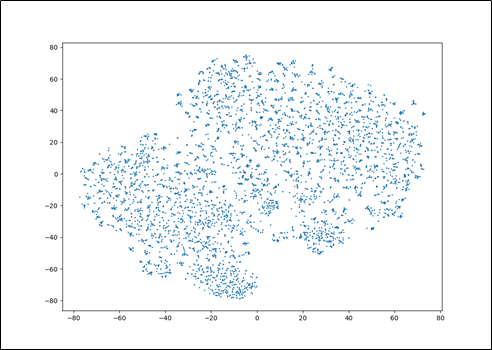
\includegraphics[width=5.09in,height=3.6in]{./media/image8.png}
		\caption{TSNE Analysis on FaceNet Embeddings}
		\label{fig:TSNE_Analysis_on_FaceNet_Embeddings}
	\end{Center}
\end{figure}


%%%%%%%%%%%%%%%%%%%% Figure/Image No: 4 Ends here %%%%%%%%%%%%%%%%%%%%

\\

\end{Center}\par


\vspace{\baselineskip}
\begin{Center}


%%%%%%%%%%%%%%%%%%%% Figure/Image No: 5 starts here %%%%%%%%%%%%%%%%%%%%

\begin{figure}[H]
	\begin{Center}
		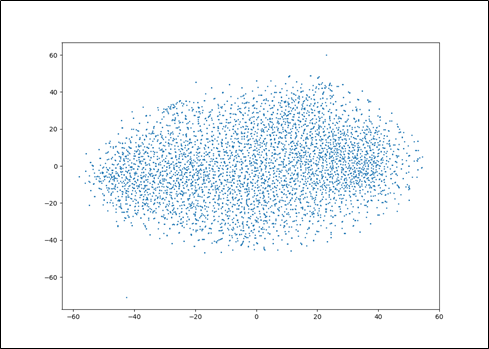
\includegraphics[width=5.04in,height=3.6in]{./media/image3.png}
		\caption{TSNE Analysis on DR-GAN Embeddings}
		\label{fig:TSNE_Analysis_on_DRGAN_Embeddings}
	\end{Center}
\end{figure}


%%%%%%%%%%%%%%%%%%%% Figure/Image No: 5 Ends here %%%%%%%%%%%%%%%%%%%%

\\

\end{Center}\par

\section*{3\hspace*{10pt}APPROXIMATE NEAREST NEIGHBOURS}
\addcontentsline{toc}{section}{3\hspace*{10pt}APPROXIMATE NEAREST NEIGHBOURS}
\begin{justify}
Nearest neighbor search (NNS) is the optimization problem of finding the point in a given set that is closest (or most similar) to a given point. Closeness is typically expressed in terms of a dissimilarity function: the less similar the objects, the larger the function values. In some applications it may be acceptable to retrieve a "good guess" of the nearest neighbor. In those cases, we can use an algorithm which doesn't guarantee to return the actual nearest neighbor in every case, in return for improved speed or memory savings. These algorithms are called Approximate Nearest Neighbour Search (ANN).
\end{justify}\par

\begin{justify}
The recognition subtask involves comparing the embedding of the face obtained with that of faces stored in a database. This subtask returns the ID of the person the face resembles the closest to, thereby recognizing the person. The database typically stores the face embeddings rather than the images of the faces themselves. The comparison is done by an ANN.
\end{justify}\par

In this report, I have benchmarked various ANN algorithms on the basis of queries executed versus Time. This benchmarking has been done on the FaceNet embeddings \cite{schroff2015facenet} . The ANN algorithms either have a python wrapper, a python package or were cloned from Github. Moreover, some ANN algorithms support batch processing.\par

\section*{4\hspace*{10pt}PROPOSED ARCHITECTURE}
\addcontentsline{toc}{section}{4\hspace*{10pt}PROPOSED ARCHITECTURE}



%%%%%%%%%%%%%%%%%%%% Figure/Image No: 6 starts here %%%%%%%%%%%%%%%%%%%%

\begin{figure}[H]
	\begin{FlushLeft}		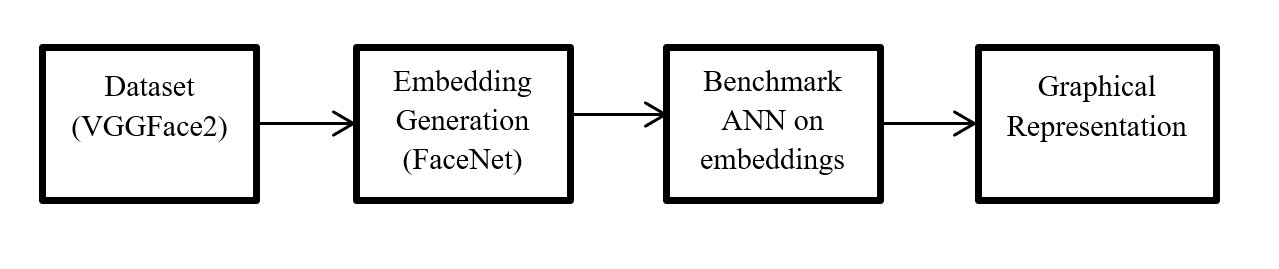
\includegraphics[width=6.27in,height=1.32in]{./media/image1.png}
		\caption{Report Implementation Overview}
		\label{fig:Report_Implementation_Overview}
	\end{FlushLeft}\end{figure}


%%%%%%%%%%%%%%%%%%%% Figure/Image No: 6 Ends here %%%%%%%%%%%%%%%%%%%%

\\

\begin{justify}
For the first part of this report two sets of embeddings have been generated for 5000 test images of VGGFace2 \cite{cao2018vggface2}. These 5000 images include 10 images each of 500 people. The two sets of embeddings are the FaceNet embeddings \cite{schroff2015facenet}  and DR-GAN’s pose invariant embeddings. FaceNet embeddings \cite{schroff2015facenet}  have been generated using a Python library of the same. On the other hand, DR-GAN’s embeddings have been generated using the demo test code on their official site.
\end{justify}\par

\begin{justify}
After the demo of the embedding, we have benchmarked 20 ANN algorithms on the basis of queries executed versus Time. This benchmarking has been done on the FaceNet embeddings \cite{schroff2015facenet}  generated in the previous part. The ANN algorithms either have a python wrapper, a python package or were cloned from Github. Moreover, some ANN algorithms support batch processing. Some of the older ANNs which were implemented in Python 2 were converted to equivalent Python 3 code using Python 2to3 refactoring tool. This benchmarking has been done on Google Colab.
\end{justify}\par


\section*{5\hspace*{10pt}IMPLEMENTATION}
\addcontentsline{toc}{section}{5\hspace*{10pt}IMPLEMENTATION}
\subsection*{5.1\ \ \ \ \ \  Platforms and Technologies}
\addcontentsline{toc}{subsection}{5.1\ \ \ \ \ \  Platforms and Technologies}
Google Colaboratory - It is a free Jupyter notebook environment that runs in the cloud and stores the notebooks on Google Drive. The implementation is done on Google Colaboratory (Colab) under Python 3 environment.\par

\subsection*{5.2\ \ \ \ \ \  Python Libraries}
\addcontentsline{toc}{subsection}{5.2\ \ \ \ \ \  Python Libraries}

\begin{itemize}
	\item \textbf{Core Libraries}
    \begin{itemize}
    	\item Time - To benchmark ANN libraries.
    	\item numpy - To store N-dimensional array objects.
    	\item pandas - To store face embeddings in dataframe object.
    	\item sklearn
    	    \begin{enumerate}
    	        \item It has 3 NNS Algorithms - KDTree, Ball Tree and Brute Method.
    	        \item It has t-SNE Algorithm \cite{maaten2008visualizing} . 
    	    \end{enumerate}
    	\item 2to3 - It is a refactoring tool to convert Python 2 to Python 3 code.
    	\item keras\_facenet - To generate FaceNet face embeddings from a face image.
    	\item Matplotlib - To visualize performance of ANN libraries.
    \end{itemize}
	\item \textbf{ANN Python Libraries }
    \begin{itemize}
    	\item annoy \cite{annoy}
    	\item nearpy \cite{lshhashes}
    	\item ngt \cite{Iwasaki2016PrunedBK,iwasaki2018optimization}
    	\item pyflann \cite{muja2009flann}
    	\item mrpt \cite{hyvonen2015fast}
    	\item pynndescent \cite{dong2011efficient}
    	\item faiss \cite{JDH17}
    	\item rpforest \cite{inproceedings}
    	\item hnswlib \cite{malkov2018efficient}
    	\item nmslib - hnsw \cite{malkov2018efficient}, sw-graph, napp \cite{tellez2011succinct}
    	\item n2 \cite{malkov2018efficient}
    	\item panns \cite{panns}
    	\item kgraph \cite{dong2011efficient}
    	\item DolphinnPy \cite{dolphinn}
    	\item FALCONN \cite{andoni2015practical}
    	\item nanopq \cite{5432202,6678503}
    	\item sklearn - KDTree \cite{panigrahy2008improved}, BallTree \cite{dolatshah2015ball}, Brute
    \end{itemize}
	\item \textbf{Github}
    \begin{itemize}
    	\item DR-GAN - To generate DR-GAN embeddings of face images.  \cite{tran2017disentangled} 
    \end{itemize}
\end{itemize}\par


\vspace{\baselineskip}


\subsection*{5.3\ \ \ \ \ \  Source Code}
\addcontentsline{toc}{subsection}{5.3\ \ \ \ \ \  Source Code}
\begin{Center}


%%%%%%%%%%%%%%%%%%%% Figure/Image No: 7 starts here %%%%%%%%%%%%%%%%%%%%

\begin{figure}[H]
	\begin{Center}
		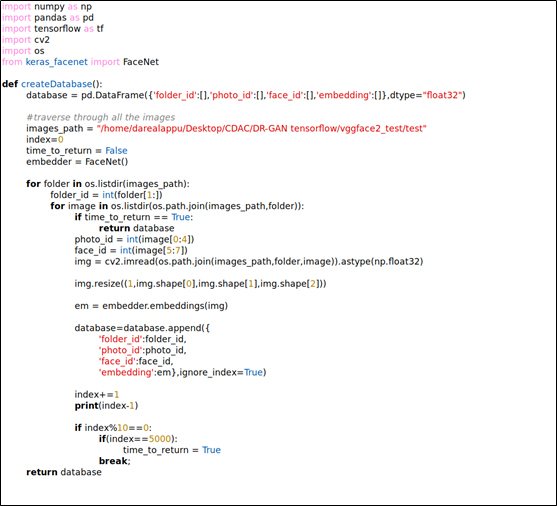
\includegraphics[width=5.8in,height=5.27in]{./media/image9.png}
		\caption{Source Code for FaceNet Embedding Generation}
		\label{fig:Source_Code_for_FaceNet_Embedding_Generation}
	\end{Center}
\end{figure}


%%%%%%%%%%%%%%%%%%%% Figure/Image No: 7 Ends here %%%%%%%%%%%%%%%%%%%%

\\

\end{Center}\par

\begin{justify}
This Python 3 script was used to create a database which contains FaceNet Embeddings of 5,000 faces. 10 images each were selected for 500 persons. This database was subsequently saved as a CSV file as $``$database.csv$"$ . A similar Python 3 script was used to create a database of DR-GAN Embeddings  \cite{tran2017disentangled}  as well
\end{justify}\par

\begin{Center}


%%%%%%%%%%%%%%%%%%%% Figure/Image No: 8 starts here %%%%%%%%%%%%%%%%%%%%

\begin{figure}[H]
	\begin{Center}
		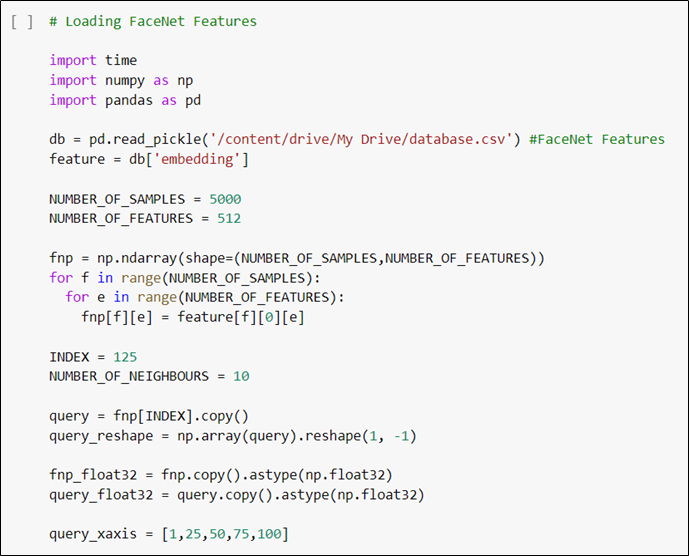
\includegraphics[width=6.27in,height=5.06in]{./media/image4.png}
		\caption{Source Code for Retrieving FaceNet Embeddings}
		\label{fig:Source_Code_for_Retrieving_FaceNet_Embeddings}
	\end{Center}
\end{figure}


%%%%%%%%%%%%%%%%%%%% Figure/Image No: 8 Ends here %%%%%%%%%%%%%%%%%%%%

\\

\end{Center}\par

\begin{justify}
This Python 3 Cell in Google Colaboratory Notebook was used to load the FaceNet Embeddings  \cite{schroff2015facenet}  from $``$database.csv$"$  and initialize various other parameters. A similar cell was used for DR-GAN Embeddings \cite{tran2017disentangled}  as well.
\end{justify}\par

\begin{Center}


%%%%%%%%%%%%%%%%%%%% Figure/Image No: 9 starts here %%%%%%%%%%%%%%%%%%%%

\begin{figure}[H]
	\begin{Center}
		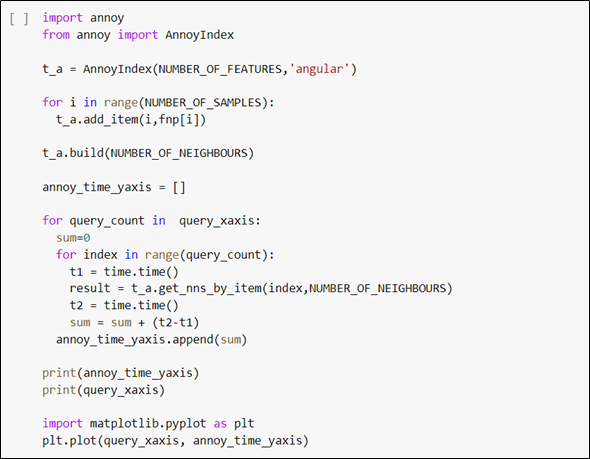
\includegraphics[width=6.15in,height=4.78in]{./media/image10.png}
		\caption{Benchmarking ANN with batch processing}
		\label{fig:Benchmarking_ANN_with_batch_processing}
	\end{Center}
\end{figure}


%%%%%%%%%%%%%%%%%%%% Figure/Image No: 9 Ends here %%%%%%%%%%%%%%%%%%%%

\\

\end{Center}\par

\begin{justify}
This Python 3 Cell in Google Colaboratory Notebook is an example of the benchmarking of an ANN which does not facilitate batch processing.
\end{justify}\par

\begin{Center}


%%%%%%%%%%%%%%%%%%%% Figure/Image No: 10 starts here %%%%%%%%%%%%%%%%%%%%

\begin{figure}[H]
	\begin{Center}
		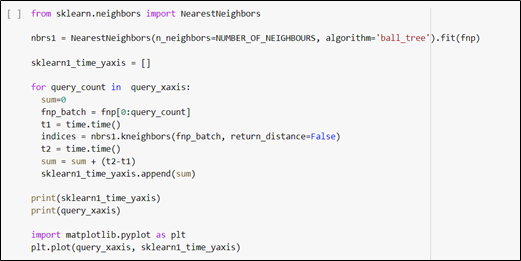
\includegraphics[width=5.43in,height=2.72in]{./media/image7.png}
		\caption{Benchmarking ANN without batch processing}
		\label{fig:Benchmarking_ANN_without_batch_processing}
	\end{Center}
\end{figure}


%%%%%%%%%%%%%%%%%%%% Figure/Image No: 10 Ends here %%%%%%%%%%%%%%%%%%%%


\end{Center}\par

\begin{justify}
This Python 3 Cell in Google Colaboratory Notebook is an example of the benchmarking of an ANN which facilitates batch processing.
\end{justify}\par

\section*{6\hspace*{10pt}RESULT AND ANALYSIS}
\addcontentsline{toc}{section}{6\hspace*{10pt}RESULT AND ANALYSIS}
\begin{justify}
20 ANN libraries in Python 3 have been benchmarked on FaceNet embeddings \cite{schroff2015facenet}  on 5000 images of VGGFace2 dataset \cite{cao2018vggface2} successfully and the results are tabulated below:
\end{justify}\par



%%%%%%%%%%%%%%%%%%%% Table No: 2 starts here %%%%%%%%%%%%%%%%%%%%


\begin{table}[H]
 			\centering
\begin{tabular}{p{6.07in}}
\hline
%row no:1
\multicolumn{1}{|p{6.07in}|}{
	\begin{Center}
		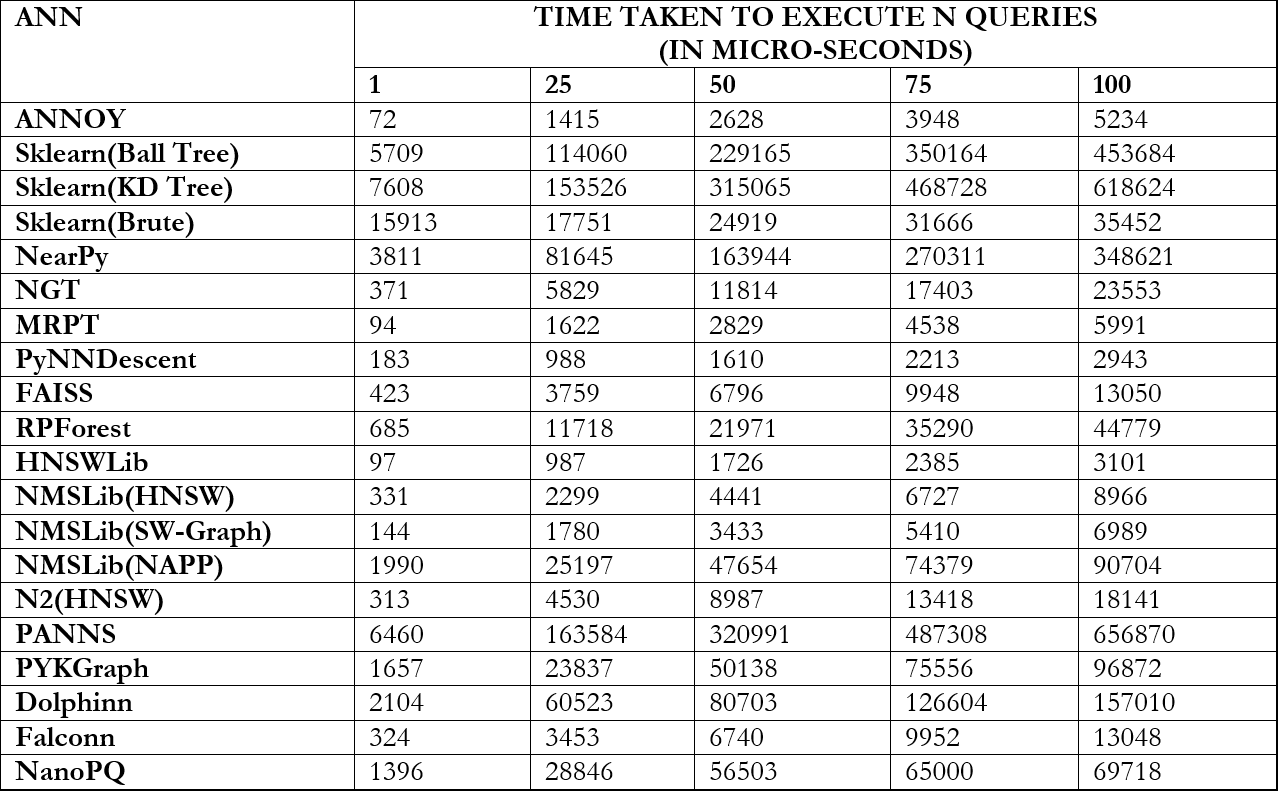
\includegraphics[scale=0.25]{./media/image11.png}
	\end{Center}
} \\
\hhline{-}

\end{tabular}\caption{ANN Benchmarks}
\label{tab:ANN Benchmarks}

 \end{table}


%%%%%%%%%%%%%%%%%%%% Table No: 2 ends here %%%%%%%%%%%%%%%%%%%%

\setlength{\parskip}{0.0pt}
\begin{FlushLeft}

\end{FlushLeft}\par


\vspace{\baselineskip}
\setlength{\parskip}{12.0pt}


%%%%%%%%%%%%%%%%%%%% Figure/Image No: 11 starts here %%%%%%%%%%%%%%%%%%%%

\begin{figure}[H]
	\begin{FlushLeft}		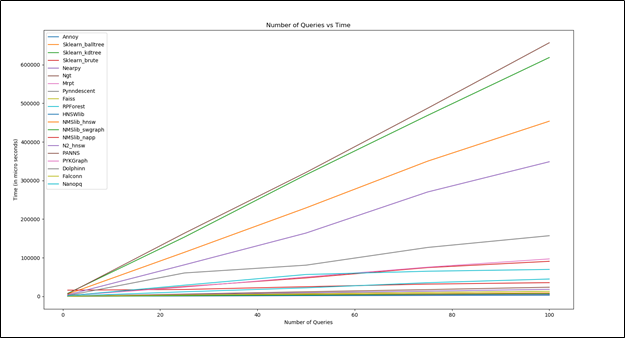
\includegraphics[scale=0.75]{./media/image5.png}
		\caption{Queries vs Time graph}
		\label{fig:Queries_vs_Time_graph}
	\end{FlushLeft}\end{figure}


%%%%%%%%%%%%%%%%%%%% Figure/Image No: 11 Ends here %%%%%%%%%%%%%%%%%%%%

\\

\section*{7\hspace*{10pt}CONCLUSION AND FUTURE SCOPE}
\addcontentsline{toc}{section}{7\hspace*{10pt}CONCLUSION AND FUTURE SCOPE}
\subsection*{7.1\ \ \ \ \ \  Conclusion}
\addcontentsline{toc}{subsection}{7.1\ \ \ \ \ \  Conclusion}
The results generated establish that while ANNOY ANN is the fastest ANN for a single query, PyNNDescent delivers the fastest results for multiple queries, given that it can facilitate batch processing as well. From the results, it is noted that for single queries, ANNOY \cite{annoy} (72 ms) gives us 23\% boost over the immediate runner-up MRPT \cite{hyvonen2015fast} (94 ms), and is 221 times faster than the slowest NNS, Brute force method of SKLearn. For Multiple Queries, Pynndescent  \cite{dong2011efficient} delivers the fastest results (2943 ms for 100 queries). It is followed closely by HNSWLib \cite{malkov2018efficient} benchmarked at 3101 ms for 100 queries.\par
Face Recognition is an active area of research and making it more suited for real time application still proves to be a challenging task. This report provides an insight on generation of face embeddings and analysis of performance of various Approximate Nearest Neighbour Libraries.  The results generated will help developers to choose a suitable ANN for their Face Recognition Pipeline.\par

 \par

\subsection*{7.2\ \ \ \ \ \  Future Scope}
\addcontentsline{toc}{subsection}{7.2\ \ \ \ \ \  Future Scope}
\begin{justify}
Even though the results generated are satisfactory, to make this project more comprehensive, the following points can be added.
\end{justify}\par

\setlength{\parskip}{0.0pt}
\begin{itemize}
	\item Include more Deep Learning Models for Embedding Generators.\par

	\item Include ANN algorithms written in Python2 by converting their code to Python3 and further optimise their performance with the new features of Python3.\par

	\item A larger Embedding Dataset can be generated to capture the performance of ANN more accurately.
\end{itemize}\par

\addcontentsline{toc}{section}{\hspace*{10pt}REFERENCES}
\newpage
\printbibliography

\setlength{\parskip}{6.0pt}


 %%%%%%%%%%%%  Starting New Page here %%%%%%%%%%%%%%

\newpage

\vspace{\baselineskip}
\vspace{\baselineskip}
\begin{Center}
\textbf{\textsc{\uline{Appendix – D}}}
\end{Center}\par

\begin{Center}
{\fontsize{14pt}{16.8pt}\selectfont \textbf{\uline{Log Book }}\par}
\end{Center}\par

{\fontsize{14pt}{16.8pt}\selectfont \textbf{Roll No.\tab \tab \tab :- 31106}\par}\par

{\fontsize{14pt}{16.8pt}\selectfont \textbf{Name of the Student\tab :- Apoorv Dixit}\par}\par

{\fontsize{14pt}{16.8pt}\selectfont \textbf{Name\ of\ the Guide   \tab :- Prof. P.S.Vidap}\par}\par

{\fontsize{14pt}{16.8pt}\selectfont \textbf{Seminar\ Title\   \tab \tab :- Similarity Search Algorithms on Embeddings in Face Recognition}\par}\par


\vspace{\baselineskip}

\vspace{\baselineskip}


%%%%%%%%%%%%%%%%%%%% Table No: 3 starts here %%%%%%%%%%%%%%%%%%%%


\begin{table}[H]
 			\centering
\begin{tabular}{p{0.56in}p{0.75in}p{2.31in}p{1.85in}}
\hline
%row no:1
\multicolumn{1}{|p{0.56in}}{\textbf{Sr. No.}} & 
\multicolumn{1}{|p{0.75in}}{\textbf{Date}} & 
\multicolumn{1}{|p{2.31in}}{\textbf{Details of Discussion/ Remarks}} & 
\multicolumn{1}{|p{1.85in}|}{\textbf{Signature of guide / Seminar Incharge}} \\
\hhline{----}
%row no:2
\multicolumn{1}{|p{0.56in}}{1.} & 
\multicolumn{1}{|p{0.75in}}{} & 
\multicolumn{1}{|p{2.31in}}{} & 
\multicolumn{1}{|p{1.85in}|}{} \\
\hhline{----}
%row no:3
\multicolumn{1}{|p{0.56in}}{2.} & 
\multicolumn{1}{|p{0.75in}}{} & 
\multicolumn{1}{|p{2.31in}}{} & 
\multicolumn{1}{|p{1.85in}|}{} \\
\hhline{----}
%row no:4
\multicolumn{1}{|p{0.56in}}{3.} & 
\multicolumn{1}{|p{0.75in}}{} & 
\multicolumn{1}{|p{2.31in}}{} & 
\multicolumn{1}{|p{1.85in}|}{} \\
\hhline{----}
%row no:5
\multicolumn{1}{|p{0.56in}}{4.} & 
\multicolumn{1}{|p{0.75in}}{} & 
\multicolumn{1}{|p{2.31in}}{} & 
\multicolumn{1}{|p{1.85in}|}{} \\
\hhline{----}
%row no:6
\multicolumn{1}{|p{0.56in}}{5.} & 
\multicolumn{1}{|p{0.75in}}{} & 
\multicolumn{1}{|p{2.31in}}{} & 
\multicolumn{1}{|p{1.85in}|}{} \\
\hhline{----}
%row no:7
\multicolumn{1}{|p{0.56in}}{6.} & 
\multicolumn{1}{|p{0.75in}}{} & 
\multicolumn{1}{|p{2.31in}}{} & 
\multicolumn{1}{|p{1.85in}|}{} \\
\hhline{----}
%row no:8
\multicolumn{1}{|p{0.56in}}{7.} & 
\multicolumn{1}{|p{0.75in}}{} & 
\multicolumn{1}{|p{2.31in}}{} & 
\multicolumn{1}{|p{1.85in}|}{} \\
\hhline{----}
%row no:9
\multicolumn{1}{|p{0.56in}}{8.} & 
\multicolumn{1}{|p{0.75in}}{} & 
\multicolumn{1}{|p{2.31in}}{} & 
\multicolumn{1}{|p{1.85in}|}{} \\
\hhline{----}
%row no:10
\multicolumn{1}{|p{0.56in}}{9.} & 
\multicolumn{1}{|p{0.75in}}{} & 
\multicolumn{1}{|p{2.31in}}{} & 
\multicolumn{1}{|p{1.85in}|}{} \\
\hhline{----}
%row no:11
\multicolumn{1}{|p{0.56in}}{10.} & 
\multicolumn{1}{|p{0.75in}}{} & 
\multicolumn{1}{|p{2.31in}}{} & 
\multicolumn{1}{|p{1.85in}|}{} \\
\hhline{----}

\end{tabular}
 \end{table}


%%%%%%%%%%%%%%%%%%%% Table No: 3 ends here %%%%%%%%%%%%%%%%%%%%

 \par

 \par


\vspace{\baselineskip}

\vspace{\baselineskip}
{\fontsize{14pt}{16.8pt}\selectfont \textbf{Student\ Signature\ \ \ \ \ \ \ \ \ \ \ \ \ \ \ \ \ \ \ \ \ \ \ \ \ \ \ \ \ \ \ \ \ \ \ \ \ \ \ \ \ \ \ \ \ \ \ \ \ \ \ \ \ \ \ \ \ \ \ \ \   Guide Signature}\par}\par

\begin{justify}
 
\end{justify}\par


\vspace{\baselineskip}

\end{document}